\section{Métricas e interpretación de los cinco modelos}
\label{sec:comparacion-modelos}
\subsection{Resultados con geometría original}
Los cinco regresores utilizan A, nueve características efectivas y las mismas particiones. La Tabla~\ref{tab:modelos} permite comparar funciones lineales regularizadas, modelos de similitud y conjuntos de árboles sin cambiar simultáneamente las entradas. Los parámetros son fijos; las métricas describen las configuraciones ejecutadas, no el óptimo de cada familia de algoritmos.
\begin{table}[htbp]
\centering\small\setstretch{1.0}
\caption{Cinco modelos con representación A: predicciones OOF por configuración.}
\label{tab:modelos}
\setlength{\tabcolsep}{4pt}
\begin{tabular}{@{}lrrrrr@{}}
\toprule
Modelo & MAE (N) & RMSE (N) & MedAE (N) & $R^2$ & Tiempo (s) \\
\midrule
\tableinput tablas/modelos.tex
\bottomrule
\end{tabular}
\par\smallskip\footnotesize Fuente: comparación de modelos existente. Los tiempos pertenecen a una ejecución separada de A--D; por ello el tiempo de Ridge difiere entre ambas tablas. Se suma ajuste y predicción de los folds.
\end{table}

\textbf{Ridge y bosque aleatorio.} El bosque obtiene MAE de 13,233~N frente a 13,247~N de Ridge: apenas 0,014~N menos. Su MedAE es menor (9,699 frente a 11,941~N), pero RMSE resulta casi idéntico (16,341 frente a 16,346~N). Mejora el error central sin reducir de forma apreciable el error cuadrático agregado. El tiempo observado del bosque es 4,126~s frente a 0,272~s de Ridge. La cercanía de los errores no demuestra superioridad estadística del conjunto de árboles.

\textbf{Elastic Net.} MAE de 13,979~N, 0,733~N mayor que Ridge. La combinación L1--L2 no aporta ventaja bajo esta configuración. No demuestra que deban eliminarse predictores ni que esa regularización sea inadecuada en general: se contrastaron parámetros fijos y no optimizados.

\textbf{SVR y proceso gaussiano.} MAE de 15,651 y 16,058~N, con RMSE de 19,096 y 19,341~N. Ambos superan el error de Ridge. Admitir relaciones no lineales mediante similitud geométrica no garantiza mejor desempeño. El resultado limita lo observado con estos núcleos y parámetros; no descarta otros ajustes o representaciones de esos algoritmos.

\subsection{Generalización entre familias}
\begin{table}[htbp]
\centering\small\setstretch{1.0}
\caption{Los mismos modelos y features al reservar familias completas.}
\label{tab:modelos-familias}
\setlength{\tabcolsep}{4pt}
\begin{tabular}{@{}lrrrrr@{}}
\toprule
Modelo & MAE (N) & RMSE (N) & MedAE (N) & $R^2$ & Tiempo (s) \\
\midrule
\tableinput tablas/modelos_familias.tex
\bottomrule
\end{tabular}
\end{table}
Elastic Net alcanza el menor MAE de este protocolo (57,113~N), seguido por Ridge (57,637~N); la diferencia es 0,524~N. Sin embargo, todos los $R^2$ son negativos. El bosque sube a 60,901~N y pierde su mínima ventaja del protocolo principal; SVR y proceso gaussiano llegan a 82,358 y 77,680~N. El orden de los modelos depende del objetivo de generalización, como muestra la Figura~\ref{fig:modelos}.

En el bosque, MedAE de 45,649~N coexiste con RMSE de 71,570~N: un error central menor puede ocultar errores grandes en otros casos. MAE se conserva como métrica principal; RMSE, MedAE y los errores por familia complementan su interpretación. Ninguna de estas arquitecturas resuelve por sí sola la transferencia a una familia excluida.
\begin{figure}[htbp]
\centering
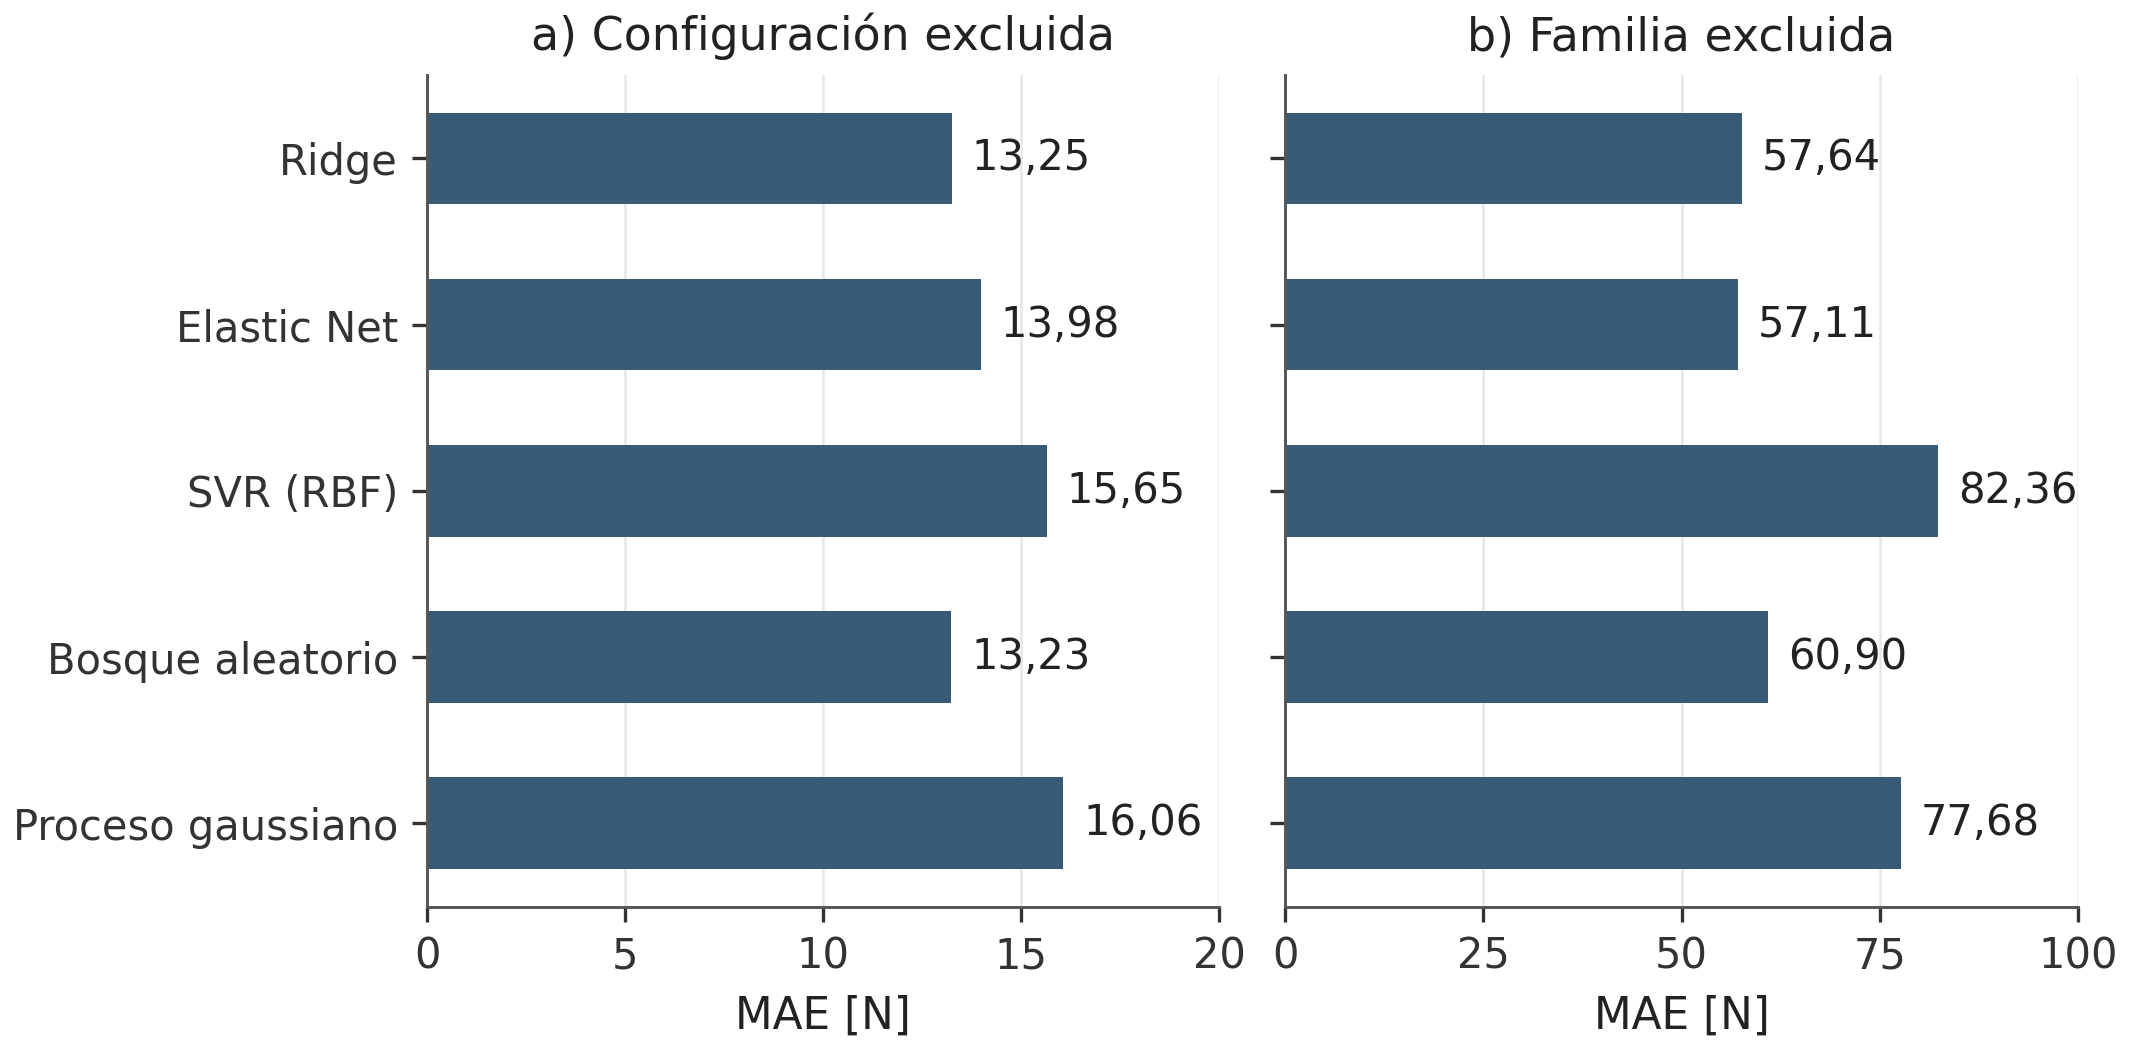
\includegraphics[width=\linewidth]{figures/05_modelos.png}
\caption{MAE de las cinco arquitecturas de regresión con geometría A. Cada panel corresponde a un protocolo y presenta su propia escala. El cambio de orden y el aumento de error obligan a distinguir configuraciones reservadas de familias completas.}
\label{fig:modelos}
\end{figure}
